%% This is file `elsarticle-template-1-num.tex',
%%
%% Copyright 2009 Elsevier Ltd
%%
%% This file is part of the 'Elsarticle Bundle'.
%% ---------------------------------------------
%%
%% It may be distributed under the conditions of the LaTeX Project Public
%% License, either version 1.2 of this license or (at your option) any
%% later version.  The latest version of this license is in
%%    http://www.latex-project.org/lppl.txt
%% and version 1.2 or later is part of all distributions of LaTeX
%% version 1999/12/01 or later.
%%
%% Template article for Elsevier's document class `elsarticle'
%% with numbered style bibliographic references
%%
%% $Id: elsarticle-template-1-num.tex 149 2009-10-08 05:01:15Z rishi $
%% $URL: http://lenova.river-valley.com/svn/elsbst/trunk/elsarticle-template-1-num.tex $
%%
\documentclass[preprint,review,times,12pt]{elsarticle}

%% Use the option review to obtain double line spacing
%% \documentclass[preprint,review,12pt]{elsarticle}

%% Use the options 1p,twocolumn; 3p; 3p,twocolumn; 5p; or 5p,twocolumn
%% for a journal layout:
%% \documentclass[final,1p,times]{elsarticle}
%% \documentclass[final,1p,times,twocolumn]{elsarticle}
%% \documentclass[final,3p,times]{elsarticle}
%% \documentclass[final,3p,times,twocolumn]{elsarticle}
%% \documentclass[final,5p,times]{elsarticle}
%% \documentclass[final,5p,times,twocolumn]{elsarticle}


\usepackage[left=1in, right=1in, top=1in, bottom=1in]{geometry}
\usepackage{graphicx}
\usepackage{amssymb}
\usepackage{amsthm}
\usepackage{amsmath}
\usepackage{lineno}
\usepackage{caption}
\usepackage{natbib}

\journal{Ecological Modelling}
\setcitestyle{authoryear,round,semicolon,sort}
\bibliographystyle{apalike}
\begin{document}
\begin{frontmatter}

\title{The performance of presence-based and process-based species distribution models under realistic conditions}

\author[NREN,CS]{Tim M. Szewczyk}
\author[CS]{Marek Petrik}
\author[NREN]{Jenica M. Allen}

\address[NREN]{Department of Natural Resources and the Environment, University of New Hampshire}
\address[CS]{Department of Computer Science, University of New Hampshire}

\begin{abstract}
Abstract here
\end{abstract}

\begin{keyword}
integral projection model; cellular automaton; virtual species; demography; niche model; mis-specification
\end{keyword}

\end{frontmatter}
\linenumbers



\section{Introduction}
\label{S:1}
% SDMs and the prevalence of occurrence-based methods (And)
Species distribution models (SDMs) have been used extensively to predict where species are expected to occur, both presently and in the future \citep{Guisan2005,Phillips2008,Elith2009,Allen2016,Araujo2019}. The majority of SDMs found in the literature are occurrence-based, using approaches such as Maxent to predict a species' distribution based on the relationship of a set of geo-referenced detections with environmental variables \citep{Elith2009}. A wide variety of techniques have been developed \citep{Elith2009,Fitzpatrick2013,Norberg2019}, with much attention in the literature to the relative strengths and weaknesses of different approaches \citep{Elith2009,Merow2014b,Fernandes2018,Norberg2019}, and resulting strategies for avoiding common biases or errors in available datasets \citep{Merow2013,Boria2014,Merow2016}. In some cases, local absence data are available as well to help inform these models \citep{Koshkina2017}. Under many conditions, these methods are highly capable of predicting current distributions CITE, and several large online databases provide easy access to adequate and ever-growing datasets CITE.

% Process-based SDMs as an alternative, including a specific example or two (But)
However, occurrence-based methods require several assumptions which may limit their use in key conservation situations. In particular, occurrence-based SDMs assume that populations are at equilibrium with the environment, such that the present distribution reflects constraints due to broad environmental conditions \citep{Elith2009}. Extrapolating to novel environmental conditions is frequently unreliable, as evidenced by the mismatches seen between the observed and predicted ranges of species in non-native continents CITE. In a world with a changing climate, the assumption of distributions at equilibrium is already invalid. Distributional shifts consistent with a warming climate have been observed in many taxa, ranging from plants \citep{Lenoir2010,Engler2011} to mammals \citep{Moritz2008a,Rowe2015} to birds \citep{Tingley2009a,Tingley2012} to moths \citep{Chen2009b}. The disparity between past occurrences and current climate will continue to increase. Process-based SDMs have been proposed as an alternative approach that may be less sensitive to these key limitations of occurrence-based SDMs \citep{Merow2011a,Evans2016,Merow2017,Cabral2017}. Rather than occurrences, process-based SDMs rely on geographically varying demographic rates, such as survival or flowering probability, to ultimately predict the distribution as an emergent property of environmentally dependent population dynamics \citep{Evans2016,Cabral2017}.

% Expected benefits of process-based SDMs (And)
Process-based SDMs are a set of highly flexible of modelling approaches which encompass individual-based and population-based methods, as well as analytical and simulation-based techniques. For example, Integral Projection Models (IPMs) incorporate effects of individual size in addition to climatic conditions to predict the intrinsic growth rate, $\lambda$, in each pixel of the landscape via demographic rates \citep{Easterling2000,Merow2017}. In contrast, cellular automata (CA) models simulate the movement of individuals across a gridded landscape, incorporating regional dispersal dynamics with local population growth based on individual-level or population-level demography \citep{Merow2011a,Szewczyk2019}. Process-based SDMs thus have several expected advantages over occurrence-based SDMs. First, process-based SDMs predict the rates of biological processes across a geographic region using regressions with environmental conditions. Consequently, there are no assumptions about equilibrium between the climate and the current distribution, but rather that the data used to fit the regressions are representative of the environmental gradient. Second, process-based SDMs predict easily interpreted and biologically meaningful quantities, such as intrinsic growth rates or abundances, as well as the underlying demographic rates and, potentially, spatially varying sensitivities. These additional parameters can help to inform applied management decisions \citep{Matzek2015,Szewczyk2019}. Third, the models are perhaps conceptually nearer to reality, representing the distribution as an emergent property of local and regional processes \citep{Merow2014b,Evans2016}.

% Benefits of occurrence-based, and the unknowns of process-based performance (But) 
There are, however, limitations and challenges with successfully implementing process-based SDMs. In stark contrast to occurrence-based SDMs, process-based SDMs have heavy data requirements \citep{Merow2014a,Evans2016}. Each demographic rate must be estimated either as a global parameter or as dependent on the environment and possibly size \citep{Merow2014a,Szewczyk2019}. Relevant rates will depend on the species, but may include annual survival probability, mean annual growth, variability in annual growth, flowering probability, mean per capita seed production, seedbank survival rates, and germination probabilities, in addition to dispersal parameters if movement between cells is included \citep{Merow2011a,Szewczyk2019}. Process-based SDMs are also structurally complex. Missing or mis-specified processes may have cascading impacts that are difficult to predict \citep{Merow2014c}. Similarly, problems and solutions resulting from common imperfections in datasets have been investigated for occurrence-based SDMs \citep{Wisz2008,Boria2014,Merow2016,Fernandes2018}. The individualized nature of process-based SDMs, with model structures based on species' life cycles \citep{Merow2011a,Merow2017,Szewczyk2019}, may render the effects and solutions of data-based problems more difficult to generalize. Thus, while process-based SDMs are intuitively appealing, it would be prudent to verify their expected benefits and appraise their resilience to errors before widespread adoption.

% Mission statement (Therefore)
Here, we directly evaluate the performance of the occurrence-based SDM Maxent and three process-based SDMs using two virtual species and multiple virtual sampling regimes. We investigate the ability of each SDM to predict the true distributions under ideal conditions, as well as under various data and modelling scenarios to represent a range of realistic challenges. Specifically, we ask: 1) Do process-based models outperform Maxent overall? 2) Are process-based or occurrence-based SDMs more susceptible to particular data deficiencies? 3) Do common modelling mis-specifications negate any improved performance otherwise observed in the process-based SDMs?




\section{Methods}
\label{S:2}
\begin{figure}
	\centering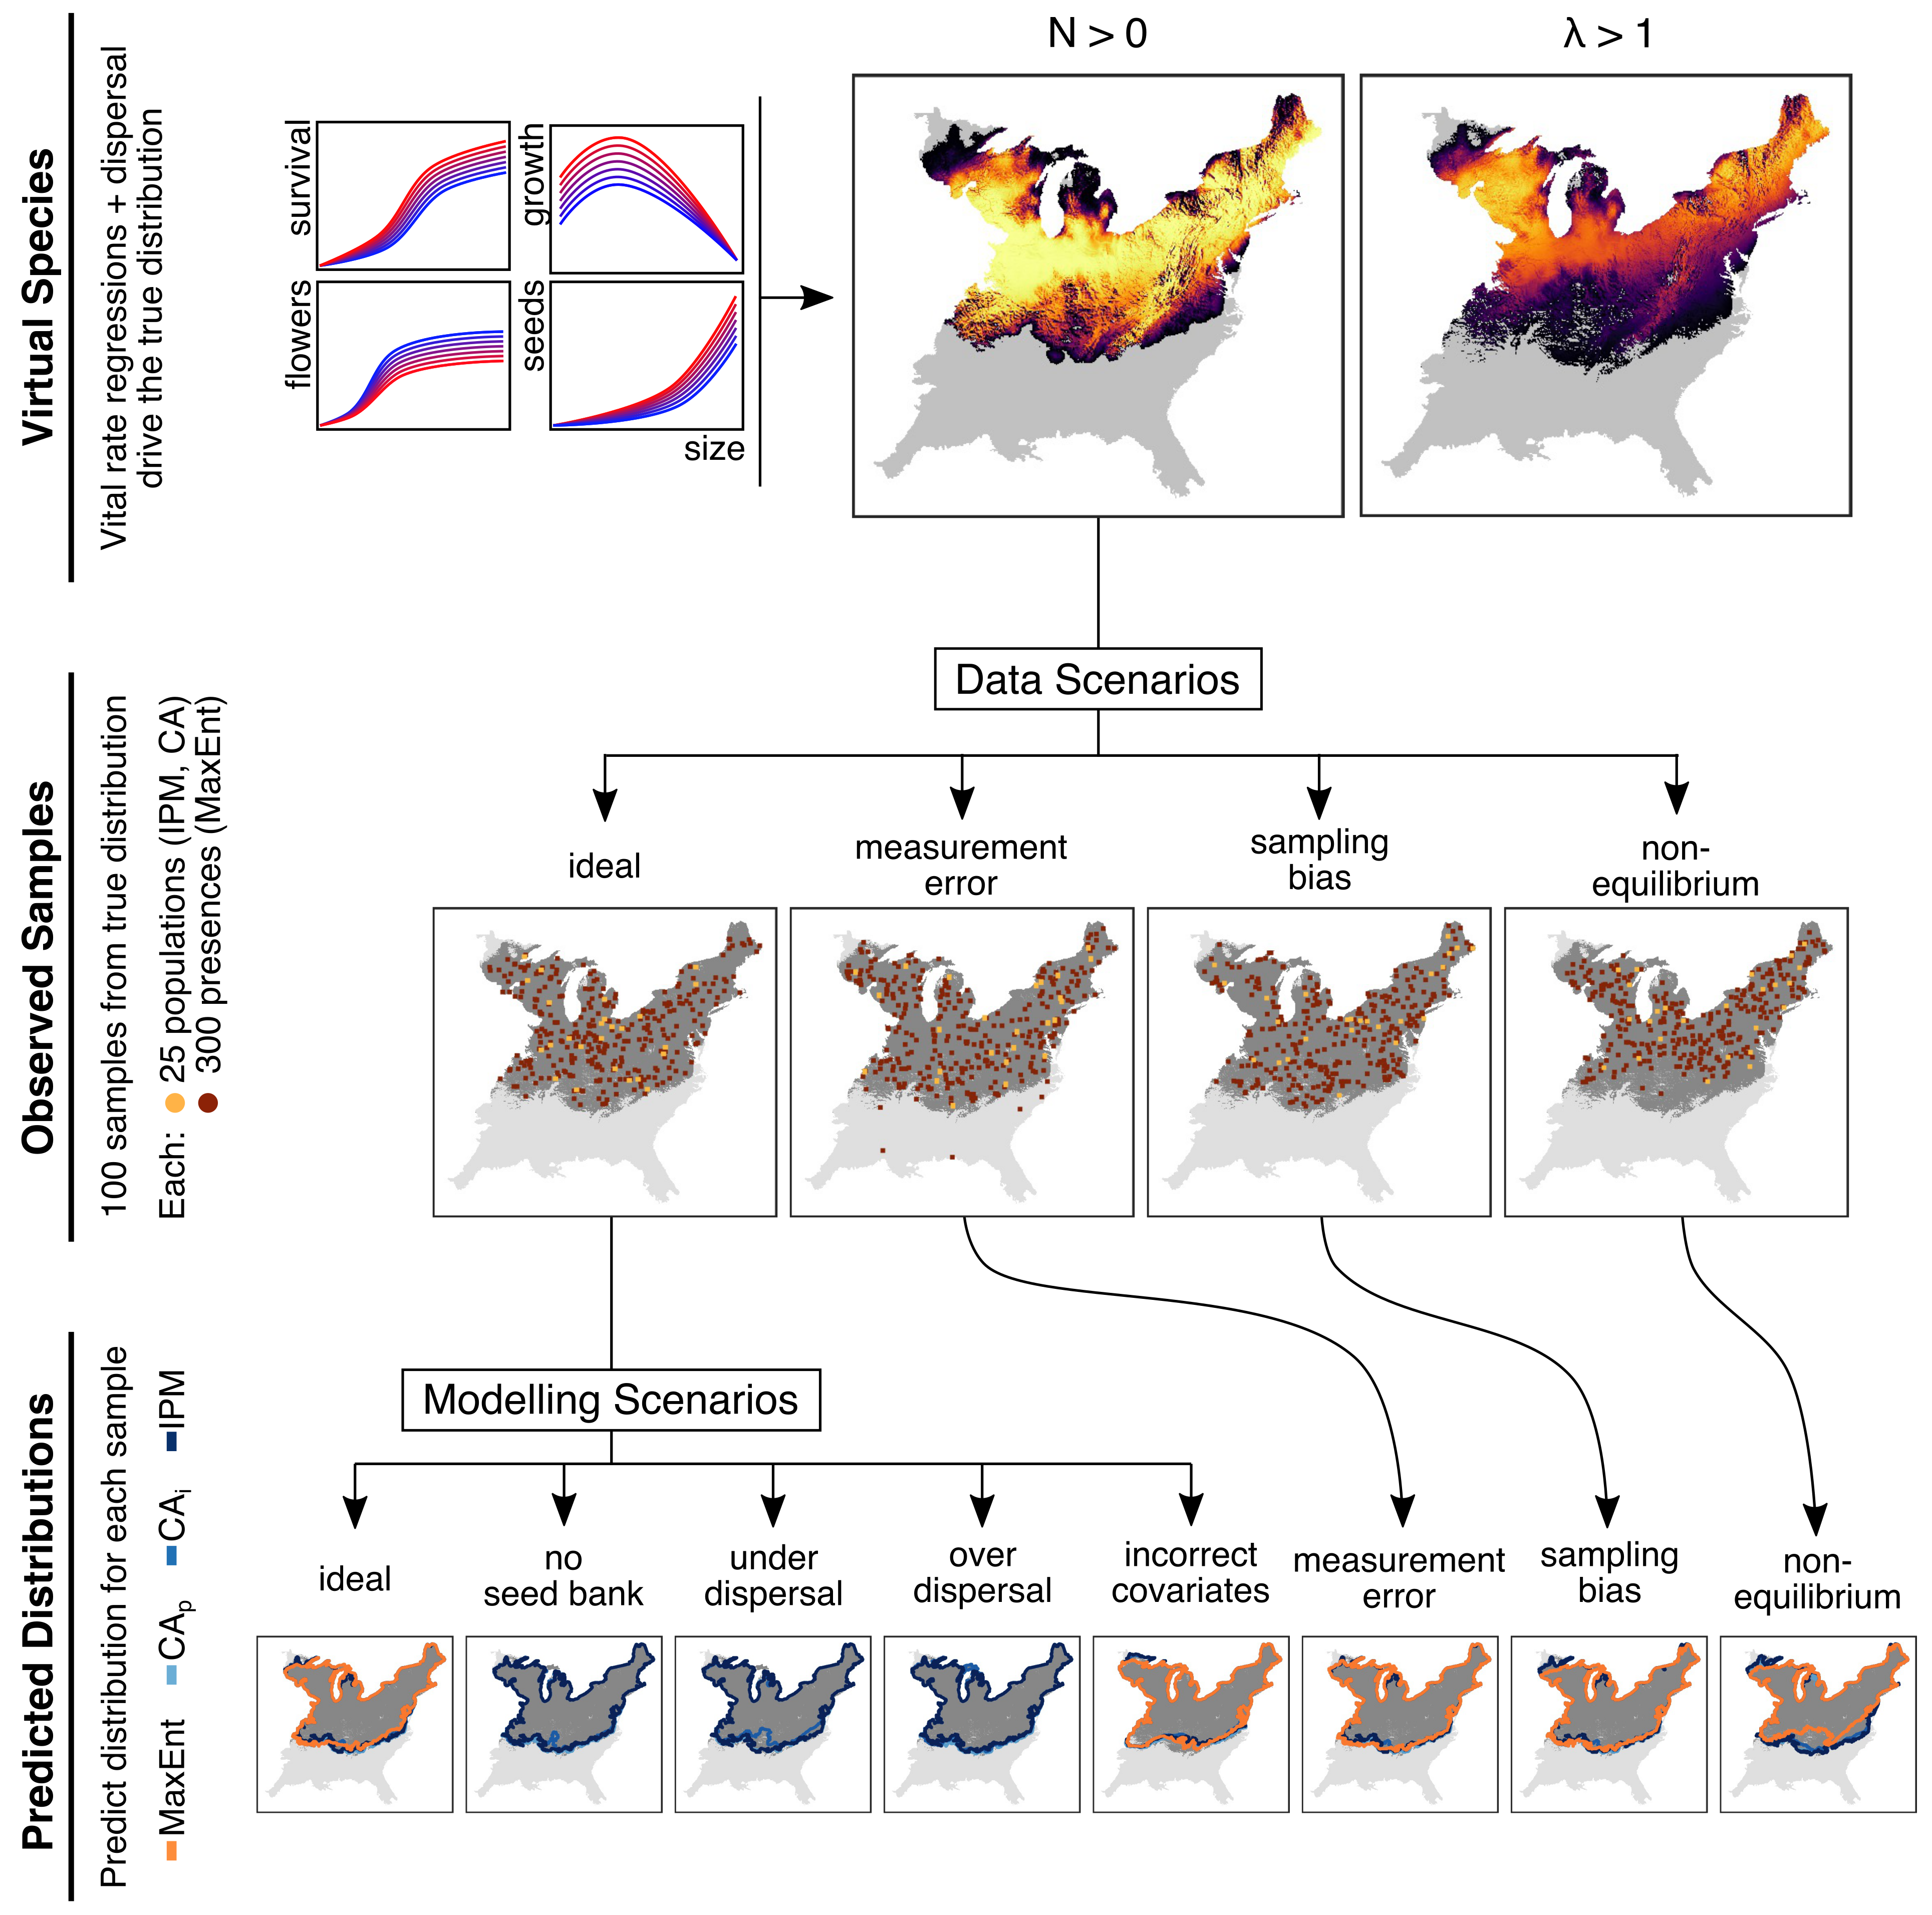
\includegraphics[width=5in]{figs/process_outline.png}
	\caption{\label{fig:outline} Simulation, sampling, and prediction process. Distributions were simulated for virtual species based on environmental effects on size-dependent vital rates and demographic processes. From the simulated distribution for each virtual species, we drew samples to parameterize four SDMs (occurrence-based: Maxent; process-based analytic: IPM; process-based stochastic: CA\textsubscript{p}, CA\textsubscript{i}). We evaluated the performance of each SDM under four sampling scenarios and four modelling scenarios.}
\end{figure}

% General outline
We evaluated the performance of four species distribution models (SDMs) in predicting the ranges of two simulated species under a variety of data quality and modelling scenarios (Fig. \ref{fig:outline}) on a gridded landscape. We compared one occurrence-based SDM (Maxent) and three process-based SDMs (Integral Projection Model: IPM; individual-level cellular automata: CA\textsubscript{i}; and population-level cellular automata: CA\textsubscript{p}). For each species under each scenario, we parameterized the SDMs using 100 samples from the true distributions. We evaluated ability of each SDM to predict the true distribution, and the relative effects of each scenario on predictive accuracy. Additional details for the virtual species, process-based models, and scenarios are included in Appendix A. All code is available online at \textless https://github.com/Sz-Tim/sdmMethodComp\textgreater.

\subsection{Species Distribution Models}
Maxent employs the machine learning technique of maximum entropy to relate a set of presences with environmental conditions, optimizing a probability surface against a background based on pseudo-absences to predict the relative suitability across the landscape for the species \citep{Phillips2008}. Maxent models were fit in the \emph{dismo} R package with a threshold of 0.95 using the logistic output with 10 replicates for each dataset. 

IPMs predict a deterministic intrinsic growth rate $\lambda$ in each cell of the landscape by integrating across a kernel based on regressions of vital rates with environmental variables and individual sizes \citep{Easterling2000,Ellner2006,Merow2014a,Merow2017}, such that: 
\begin{equation}
    n_{t+1}(z^{\prime}) = \int_{\Omega} K(z^{\prime}, z) n_t(z) dz 
\end{equation}
\begin{equation}
    K(z^{\prime}, z) = P(z^{\prime}, z) + F(z^{\prime}, z)
\end{equation}
where $z$ represents size as a continuous variable, $n$ is the distribution across sizes, $\Omega$ is the range of possible sizes, $K(z^{\prime}, z)$ is the kernel representing the probability of transitions among sizes, $P(z^{\prime}, z)$ is the growth and survival component, and $F(z^{\prime}, z)$ is the fecundity component. To compose $P(z^{\prime}, z)$, we included regressions for growth and survival. To compose $F(z^{\prime}, z)$, we included regressions for flowering probability, seed production, and germination. Additionally, we incorporated a seedbank as a discrete stage (Appendix A: Section 1.2). Short distance dispersal was implemented by adjusting $F(z^{\prime}, z)$ for cells within each short distance dispersal neighborhood to account for the increase in the propagule pressure due to seed immigrants from nearby cells as well as the decrease from seed emigrants out of each cell (Appendix A: Section 1.3). 

In contrast to analytical IPMs, CA models are simulation-based and explicitly model spatio-temporal dynamics among cells. The individual-level cellular automaton model (CA\textsubscript{i}) simulates individuals in each cell of the landscape by building on the structure of the IPM. We simulated local processes within each cell, including survival, growth, flowering, seed production, germination, and seedbank dynamics. We used identical vital rate regressions as for the IPM, but then simulated individuals and outcomes (e.g., annual survival, growth, etc.) in each cell by generating random numbers from the corresponding distributions using the expected values from the regressions. Regional processes were represented as the dispersal of seeds both within short distance dispersal neighborhoods and to a set number of random cells in the landscape. 

The population-level cellular automaton model (CA\textsubscript{p}) uses population averages to summarize similar processes, and models approximately age-structured populations which include pre-reproductive juvenile stages and a single adult stage \citep{Merow2011a,Szewczyk2019}. Seeds are similarly dispersed via short distance dispersal among nearby cells and via stochastic long distance dispersal to any cell on the landscape. All three process-based SDMs thus model local populations within each cell driven by similar demographic processes, and dispersal of seeds among cells at a more regional scale.

\subsection{Virtual Species Simulation}
We simulated two virtual species in the eastern United States, based approximately on Japanese barberry (\emph{Berberis thunbergii}), an invasive shrub with bird-dispersed seeds, and garlic mustard (\emph{Alliaria petiolata}), an invasive biennial with seeds dispersed by non-volant animals and water. Both species have previously been the focus of process-based SDMs \citep{Merow2017}. For each species, we defined relationships where vital rates were dependent on environmental variables and individual size (Fig. \ref{fig:outline}, Appendix A) on a gridded landscape spanning the Eastern Temperate Forest and Northern Forest ecozones within the United States ($\sim$5x5km resolution: 115,105 cells \citep{Omernik2014}). Vital rates included annual individual growth, annual survival, flowering probability, seed production, and germination probability. For individuals of a given size, each vital rate was determined by the response to the minimum temperature of the coldest month and the precipitation in May, following previous work \citep{Merow2017}. We calculated a mean value for each climatic variable in each cell using the CHELSA climate dataset \citep{Karger2017}. We defined the true range for each species using two methods: cells where the intrinsic growth rate $\lambda>1$ (i.e., analytic), and cells containing individuals at the end of the simulation (i.e., dynamic).

We calculated the intrinsic growth rate $\lambda$ in each cell following the methods used for IPMs, where each cell was treated as a population. Vital rate regressions and parameters were initially informed based on previous work on each species in New England, USA \citep{Merow2017}, but modified \emph{ad hoc} to generate equilibrium distributions approximating the current distribution of each species in the eastern United States. For the shrub, dispersal parameters were based on dispersal rates of similarly bird-dispersed invasive shrubs \citep{Merow2011a,Szewczyk2019}. For the biennial, short distance dispersal was decreased and long distance dispersal increased to qualitatively reflect the mode of dispersal. For the shrub, $\lambda$ was calculated in each cell as the first eigenvalue of the transition matrix constructed from the vital rate regressions (Appendix A). The two-year life cycle of the biennial required calculating $\lambda$ by iterating populations through the transition matrix until the distribution had stabilized, at which point $\lambda$ is calculated as $N_t/N_{t-1}$. Cells with $\lambda > 1$ were considered to be capable of supporting persistent populations, constituting the true $\lambda$-based definition for each species. 

To simulate populations, we initialized 10 random cells with 10 individuals, with individual sizes drawn from a uniform distribution constrained by the allowable range for each species. Then, we calculated the expected survival probability, growth rate, flowering probability, and seed production for each individual according to the same vital rate regressions used in the calculation of $\lambda$ (Appendix A). We drew random values from the appropriate distributions for each vital rate for each individual, implemented short- and long-distance dispersal of seeds according to the dispersal mode of each species, and generated new individuals in each cell from germinating seeds. Populations in each cell were subject to density dependence through reduced seedling establishment \citep{Ellner2006,Rebarber2012,Merow2014a} after the abundance exceeded a predetermined threshold. The populations were simulated through 300 years, at which point the distribution appeared stable, indicating that equilibrium had been reached. Cells with $N > 0$ in the final year were considered to be the equilibrium population, constituting the true $N$-based definition for each species. 

\subsection{Sampling and Modelling Scenarios}
To generate datasets for fitting the SDMs, we drew samples from the simulated (i.e., $N$-based) distribution for each species (Fig. \ref{fig:outline}: \emph{Observed Samples}). We evaluated four sampling scenarios: \emph{ideal}, \emph{non-equilibrium}, \emph{geographic bias}, and \emph{measurement error}. For each species, we generated 100 data sets under each sampling scenario. For Maxent, each data set consisted of presences from 300 cells \citep{Wisz2008,Allen2016,Fernandes2018}. For the process-based SDMs, each data set consisted of 25 cells \citep{Merow2017}, from which a maximum of 100 (CA\textsubscript{i}, IPM) or 1000 (CA\textsubscript{p}) individuals were sampled per cell to reflect real-world logistical limitations in measuring demographic and vital rates (Appendix A). The \emph{ideal} data sets were drawn from the true virtual species distributions at year 300 with uniform sampling probability among cells occupied by at least 5 individuals. The \emph{non-equilibrium} datasets were instead drawn from the virtual species distributions at year 100. The \emph{geographic bias} data sets were drawn from year 300, but with the sampling probability for each cell proportional to the human population density and road density. For the final data set, we imposed \emph{measurement error}. For Maxent, we replaced 3\% of the observations in each data set with random cells drawn from full landscape regardless of occupancy. For the process-based SDMs, we added error to the measurements of annual growth: $g_{obs} = Norm(g_{true}, 0.1)$; seed production: $seed_{obs} = Norm(seed_{true}, seed_{true}*0.05)$; and population abundance: $N_{obs} = Norm(N_{true}, N_{true}*0.02)$. Thus, the \emph{measurement error} scenario reflects imprecision in the data sets rather than biased measurement. 

We also evaluated four scenarios of modelling mis-specification: \emph{incorrect covariates}, \emph{no seedbank} (process-based only), \emph{over-estimated dispersal} (process-based only), \emph{under-estimated dispersal} (process-based only). Each of these mis-specifications was implemented using the \emph{ideal} datasets. For \emph{incorrect covariates}, the SDMs were fit with correlated (Appendix A) but more general climate variables (mean annual temperature, annual precipitation) rather than the more specific covariates used in the generative process and for all other scenarios (minimum temperature of the coldest month, precipitation in May). For \emph{no seedbank}, the predictive SDMs assumed that all seedlings in the sampled datasets originated from seeds produced in the same year, with complete over-winter mortality of non-germinating seeds. For \emph{over-estimated dispersal}, the maximum short distance dispersal distance was increased by 2 cells, the mean short distance dispersal distance was doubled, and the number of annual long distance dispersal events multiplied by five. For \emph{under-estimated dispersal}, the maximum short distance dispersal distance was decreased by 2 cells, the mean short distance dispersal distance was halved, and the number of annual long distance dispersal events divided by five.

For each scenario (Fig. \ref{fig:outline}), the SDMs were parameterized using the corresponding sampled datasets. As explanatory variables, we used two climatic variables (minimum temperature of the coldest month, precipitation in May) and their squares, with the exception of the \emph{incorrect covariates} scenario in which we instead used the more general variables. To select environmental covariates for each process-based SDMs, we compared all combinations of the climatic variables and their squares with the R package \emph{MuMIn} for each vital rate regression. For the CA\textsubscript{i} models and IPMs, this included regressions for annual survival, annual growth, flowering probability, seed production for flowering individuals, and germination probability. For the CA\textsubscript{p} models, the demographic rate regressions included carrying capacity, juvenile survival, adult survival (shrub only), flowering probability, seed production for flowering individuals, and germination probability. With the fitted CA\textsubscript{p} and CA\textsubscript{i} models, simulations were run for 300 years to generate predicted distributions. For the fitted IPMs, we calculated $\lambda$ in each cell.

To evaluate the performance of each SDM under each scenario, we calculated the True Skill Statistic (TSS) \citep{Allouche2006} for each of the 100 predicted distributions per scenario per SDM (Maxent: 100 datasets x 5 scenarios x 2 species = 1000 predicted distributions; CA, IPM: 100 datasets x 8 scenarios x 2 species = 1600 predicted distributions). We compared each predicted distribution to the true simulated range based on population viability (true $\lambda > 1$) and based on population presence (true $N > 0$). TSS is calculated as \emph{sensitivity} + \emph{specificity} $-$ 1, where \emph{sensitivity} is the proportion of true presences that are predicted correctly, and \emph{specificity} is the proportion of true absences that are predicted correctly, such that TSS ranges from $-1$ (all cells predicted incorrectly) to $1$ (all cells predicted correctly).

To compare TSS among SDM types overall, we used the R package \emph{dunn.test} to perform Dunn's Test of Multiple Comparisons Using Rank Sums, a non-parametric post-hoc test for pairwise comparisons following a Kruskal-Wallis test. We compared SDM performance for each definition of range boundary, using the median TSS of each SDM for each species under each scenario, restricting the analyses to scenarios applicable to all four SDMs. 






\section{Results}
\label{S:3}

% Rankings (overall, ideal)
All models performed well in recovering the true $\lambda$-based ($\lambda > 1$) and $N$-based distributions ($N>0$) for both species across all scenarios (all TSS medians $>$ 0.77), though no single model performed best universally (Fig. \ref{fig:TSSmn}). Across scenarios applicable to all four SDMs (Table \ref{table:ranks}), the IPM best predicted the $\lambda$-based distributions (\emph{P\textsubscript{IPM-CA\textsubscript{i}}}: 0.02, \emph{P\textsubscript{IPM-CA\textsubscript{p}}}: 0.01, \emph{P\textsubscript{IPM-Maxent}}: 0.01), with no significant difference between the CA models and Maxent. Similarly, the CA models best predicted the $N$-based distributions (\emph{P\textsubscript{IPM-CA\textsubscript{i}}}: \textless0.01, \emph{P\textsubscript{IPM-CA\textsubscript{p}}}: \textless0.01, \emph{P\textsubscript{Maxent-CA\textsubscript{i}}}: \textless0.01, \emph{P\textsubscript{Maxent-CA\textsubscript{p}}}: 0.02) with no significant difference between the CA models. Maxent was intermediate for both range boundaries on average (mean rank: $\lambda$-based=2.7, $N$-based=2.9), though its rank was not significantly different from the process-based model(s) that performed most poorly for each range boundary.

\begin{table}
	\centering
	\captionsetup{width=.75\textwidth}
	\begin{tabular}{l c c c c}
		\hline \\[-3.5ex]
		\textbf{SDM} & \textbf{Best} & \textbf{Mean} & \textbf{Median} & \textbf{Worst}\\
		\hline 
		\hline \\[-2.5ex]
		\multicolumn{5}{l}{\textsc{True range: $\lambda > 1$}} \\
		CA\textsubscript{p} & 2 & 2.9 & 2.5 & 4\\
		CA\textsubscript{i} & 2 & 2.9 & 3 & 4\\
		IPM & 1 & 1.5 & 1 & 4\\
		Maxent & 1 & 2.7 & 2.5 & 4\\
		[.5ex]\hline \\[-2.5ex]
		\multicolumn{5}{l}{\textsc{True range: $N > 0$}} \\
		CA\textsubscript{p} & 1 & 1.9 & 2 & 3\\
		CA\textsubscript{i} & 1 & 1.6 & 1 & 4\\
		IPM & 3 & 3.6 & 4 & 4\\
		Maxent & 1 & 2.9 & 3 & 4\\
		[.5ex]\hline \\[-2ex]
	\end{tabular}
	\caption{\label{table:ranks}Summary of ranks across species and all scenarios applicable to all four SDMs. For each scenario and species, SDMs were ranked based on the median TSS.}
\end{table}

% Effect of data issues
For Maxent, TSS decreased when fit using samples from \emph{non-equilibrium} populations, driven by smaller predicted ranges as indicated by a decrease in sensitivity (Fig. B.1) and a smaller increase in specificity (Fig. B.2). In contrast, \emph{non-equilibrium} samples had minimal effect on TSS for the CA\textsubscript{p} model, with a modest improvement for the long-lived shrub in the IPM and CA\textsubscript{i} models driven by increases in sensitivity (Fig. B.1). \emph{Measurement error} and \emph{sampling bias} had negligible effects on the process-based models, and small to moderate effects on the performance of Maxent (Fig. \ref{fig:TSSmn}, Fig. B.1, Fig. B.2). 

\begin{figure}
	\centering\includegraphics[width=5in]{figs/fig_TSS_mn+CI.jpg}
	\caption{\label{fig:TSSmn} True skill statistic (TSS) mean and 95\% confidence intervals across 100 sampled data sets for each SDM and scenario, compared to true distributions defined by $\lambda > 1$ and $N > 0$. Scenarios include: no sampling or modelling issues (ideal), sampling issues (measurement error, sampling bias, non-equilibrium), and modelling issues (incorrect covariates, no seedbank, under dispersal, over dispersal).}
\end{figure}

\begin{figure}
	\centering\includegraphics[width=\linewidth]{figs/fig_TSSvIdeal.jpg}
	\caption{\label{fig:TSSvIdeal} Effect of scenario on median true skill statistic (TSS) relative to the '\emph{ideal}' scenario. Positive values indicate improved predictive ability, while negative values indicate decreased predictive ability.}
\end{figure}

% Effect of modelling issues
Modelling with \emph{incorrect covariates} decreased performance for all SDMs, though the decline tended to be larger on the process-based SDMs. It generally had a greater impact on TSS in the shrub than the biennial species (Fig. \ref{fig:TSSvIdeal}). \emph{Incorrect covariates} did not lead to systematic over-prediction or under-prediction, but rather a decrease in both sensitivity and specificity, particularly for the process-based models (Fig. B.3, Fig. B.4). Excluding the seedbank in the process-based models had minimal effect on TSS for the shrub, but variable effects on TSS for the biennial. Relative to \emph{ideal}, all process-based models showed reduced sensitivity and increased specificity for the biennial, indicating a smaller predicted range. The IPM was generally more resistant to mis-characterized dispersal compared to the simulation-based CA\textsubscript{i} and CA\textsubscript{p} models. Underestimation of dispersal parameters led to decreased predicted ranges, and overestimation to increased predicted ranges relative to \emph{ideal}. The effects were more extreme for the biennial than for the shrub.

% Process-based predictions (lambda, N, etc)
Discrepancies in predicted $\lambda$ values were biased downward in the northern portion of the study region (Fig. \ref{fig:N_Lambda}), more strongly so for the shrub. Mirroring the effect on predicted presence, residual error was most variable and most extensive when \emph{incorrect covariates} were used. Discrepancies in predicted abundance from the CA\textsubscript{p} model showed a spatial banding of upward bias at the range margins for both species (Fig. \ref{fig:N_Lambda}), indicating a tendency to over-predict at range edges. Immediately interior to the range margin, the CA\textsubscript{p} and CA\textsubscript{i} models showed upward bias for the shrub (Fig. \ref{fig:N_Lambda}). The CA\textsubscript{p} model dramatically underestimated abundance of the long-lived shrub with \emph{non-equilibrium} datasets, despite minimal impact on predicted presence or absence. As with the IPM, using \emph{incorrect covariates} tended to result in larger error in abundance predictions for both CA\textsubscript{p} and CA\textsubscript{i}.

\begin{figure}
	\centering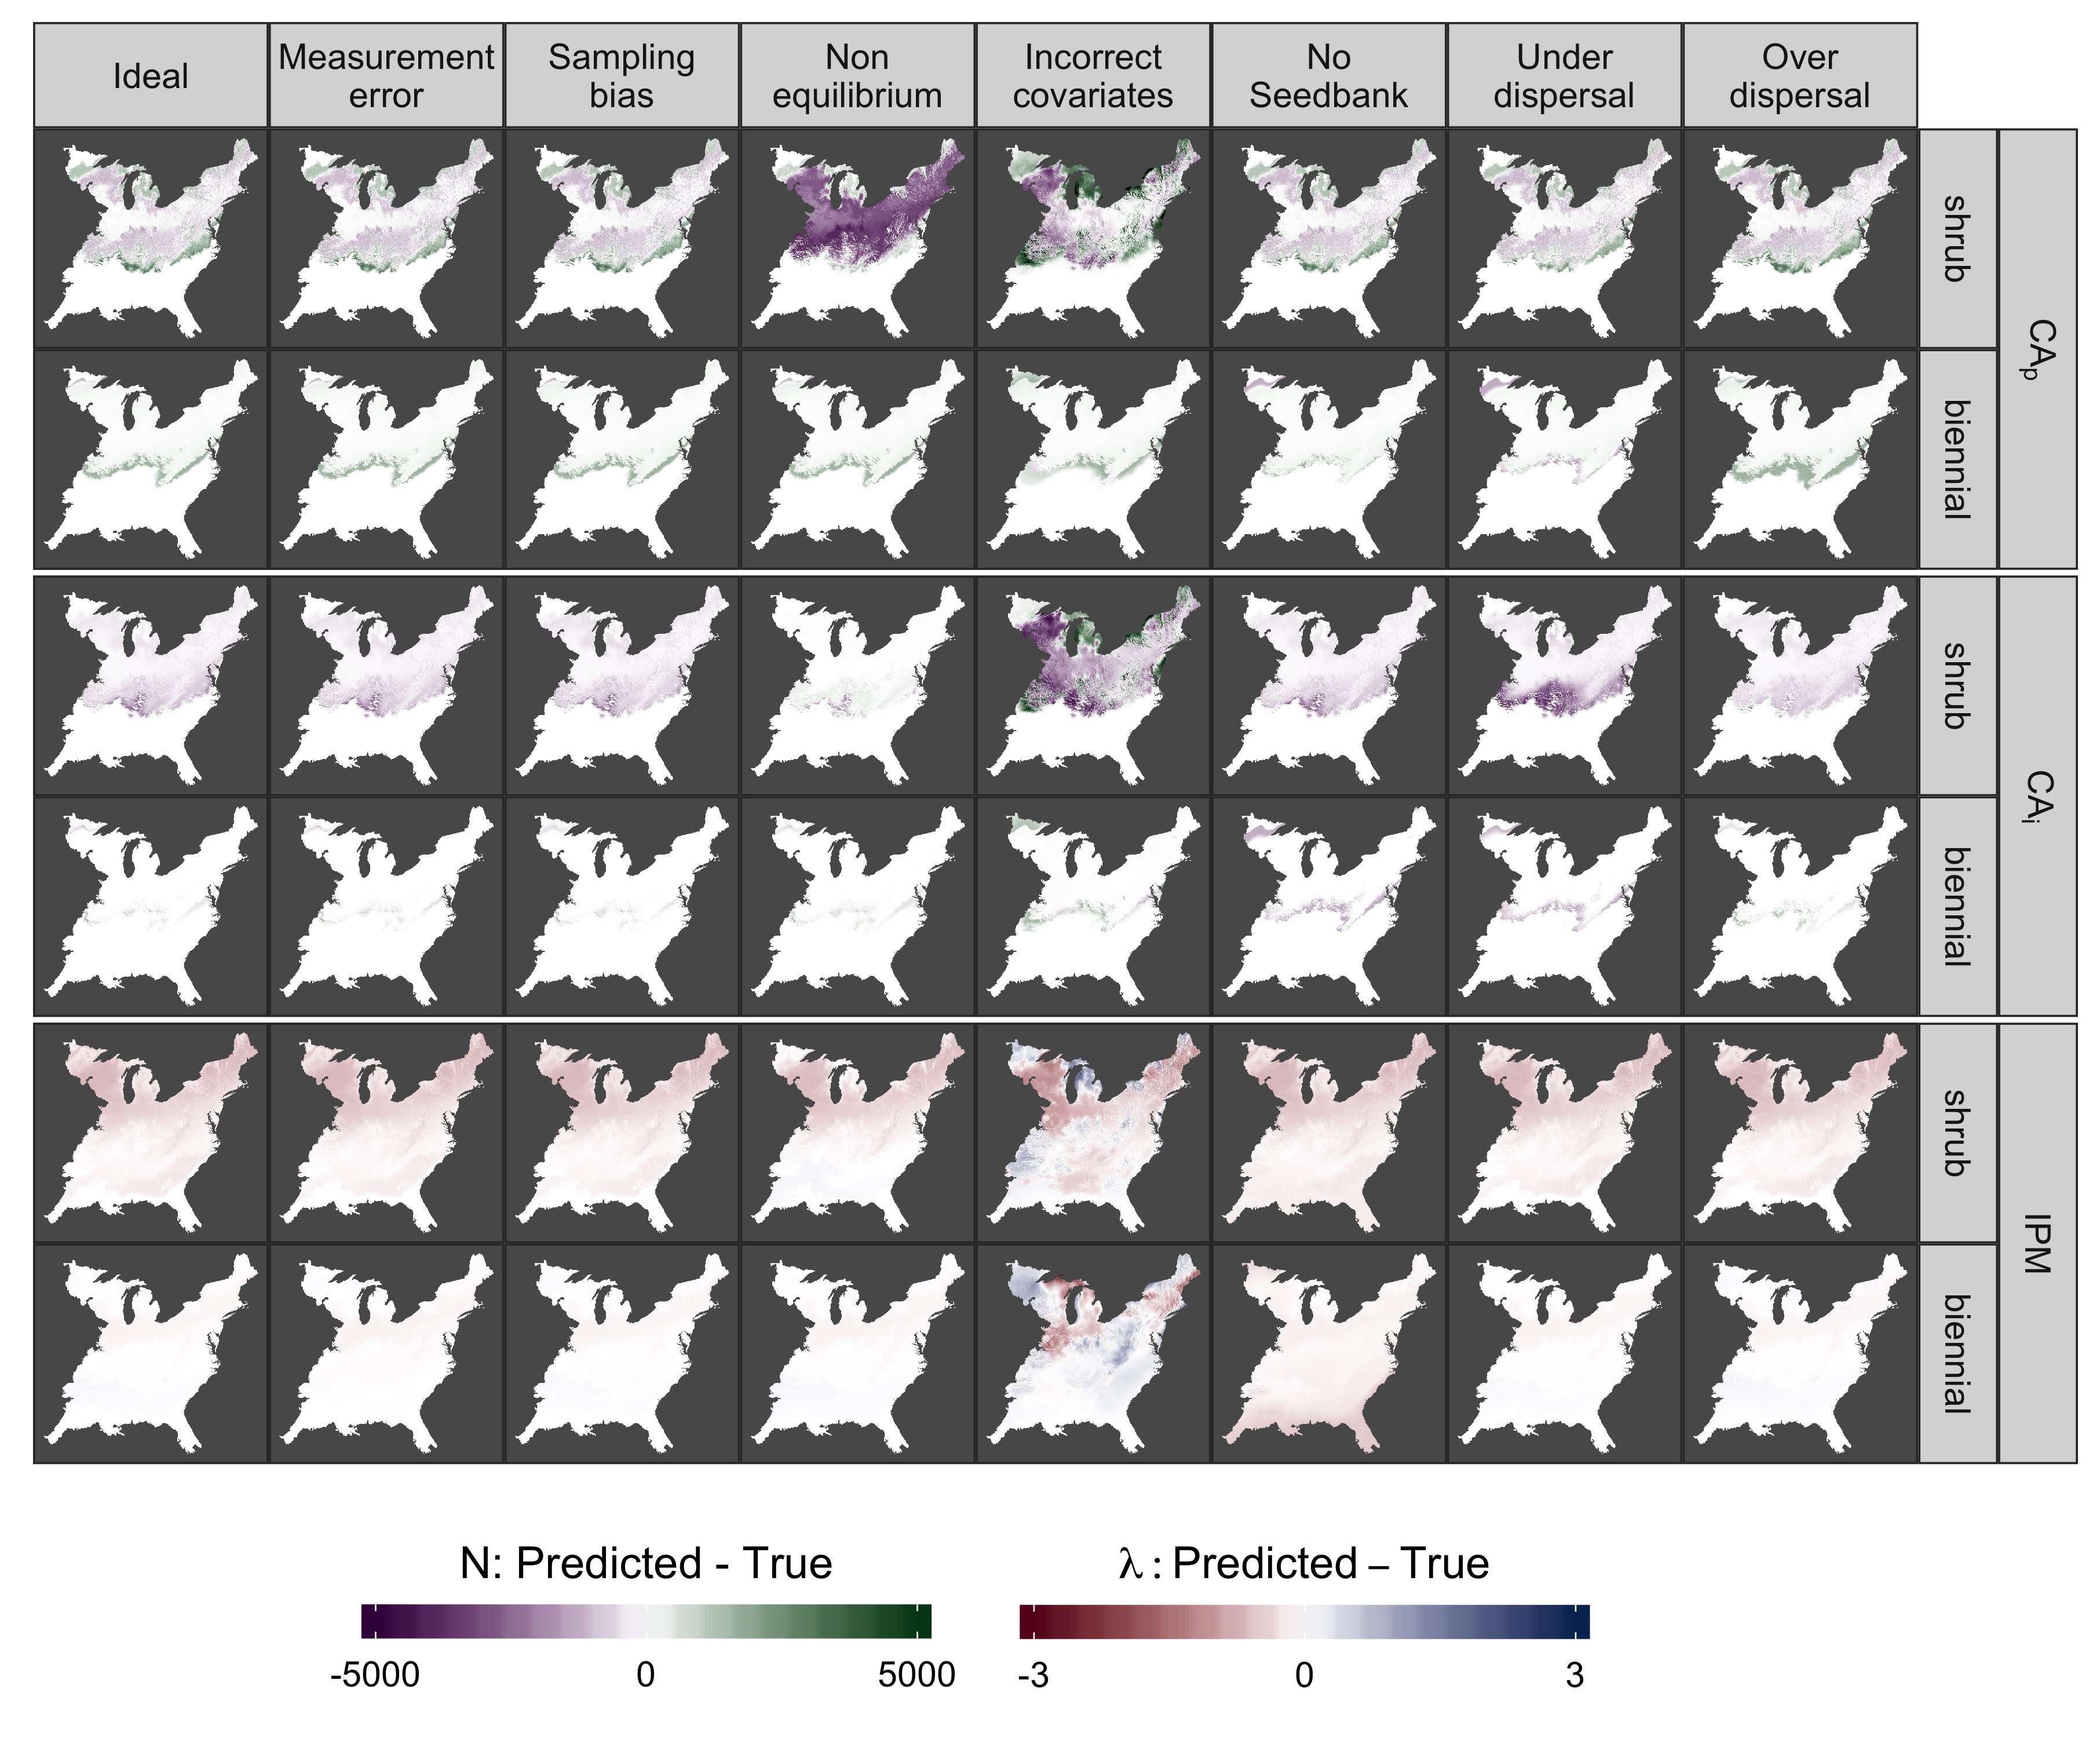
\includegraphics[width=\linewidth]{figs/map_N_Lambda.jpg}
	\caption{\label{fig:N_Lambda} Residual error in predicted $\lambda$ and $N$ under each scenario. Darker colors indicate larger residuals (under-prediction: purple, red; over-prediction: green, blue)}
\end{figure}


\section{Discussion}
\label{S:4}

% Overview
Overall, the virtual species distributions were predicted best by the process-based models when the range boundary definitions were appropriately matched. The $\lambda$-based ranges were best predicted by the IPM, and the $N$-based ranges were best predicted by the CA models, with Maxent typically intermediate in each case. Maxent showed highest sensitivity to \emph{non-equilibrium} samples. In contrast, the process-based models were relatively unaffected by \emph{non-equilibrium} samples, with moderate improvements for the longer-lived shrub. However, the process-based models were much more sensitive to the use of \emph{incorrect covariates} than Maxent. The simulation-based CA models were influenced by modelling mis-specifications, with the magnitude of the effect varying across species. While process-based SDMs indeed have many benefits over simpler occurrence-based SDMs, our results highlight the importance of accurately describing the environmental drivers impacting each vital rate. 

% Range boundaries
IPMs predict $\lambda$ in each cell of the landscape, and consequently directly predict the $\lambda$-based range boundary. Similarly, the simulation-based CA models predict abundance, thus directly predicting the $N$-based range boundary. For Maxent, the range boundary definition is less explicit. The geo-located presences used as input imply an abundance-based range, but predicted distributions are frequently constrained by a data-based threshold (e.g., relative suitability values that encapsulate 95\% of the observed data) to exclude both erroneous data and sink populations \citep{Elith2009a,Allen2016}, which implies an intent to predict a $\lambda$-based range. The practical difference between the range definitions will depend on the biology of the species. For example, the magnitude of the difference should vary with the number or distribution of marginal cells, where large areas with marginal cells may result in different patterns of occupancy. Similarly, species with high annual stochasticity in population abundances are more likely to exhibit patchier distributions due to chance local extinctions \citep{Morris2003}. Alternatively, species with high dispersal, or invasive species with a longer introduction history, are less likely to be dispersal limited, but may instead have a larger proportion of non-viable sink populations. Selection of process-based SDMs requires clearly specifying the range boundary definition in a way that occurrence-based SDMs do not.

% Process-based > Maxent under ideal conditions, and data scenarios – esp. non-equilibrium
Under ideal conditions, the process-based SDMs, when properly matched to their respective range boundary definitions, outperformed Maxent (Fig. \ref{fig:TSSmn}). The SDMs were also generally unaffected by either the addition of \emph{measurement error} or to geographic \emph{sampling bias}, though the predictions of Maxent were affected somewhat more under both scenarios. Similarly, there was little or no decrease in performance in the process-based SDMs with \emph{non-equilibrium} samples (Fig. \ref{fig:TSSvIdeal}, B.3, B.4). In fact, the individual-based models (IPM, CA\textsubscript{i}) showed marginally improved performance for the shrub, as the younger populations had a more even age distribution, allowing for more accurate estimation of the size-dependent vital rate regressions (Fig. B.5a). Because process-based SDMs aim to describe the biological processes that ultimately result in an emergent geographic distribution, care should be taken to select sample populations with an adequately broad range of sizes or ages. In contrast, the performance of Maxent declined the most in the \emph{non-equilibrium} scenario, consistent with past work (CITE). These results thus support the proposal that process-based SDMs are advantageous in situations where populations are not at equilibrium \citep{Merow2011a,Evans2016,Merow2017,Cabral2017}, such as for distributions of alien species or for future distributions as the climate continues to change. 

% But caveat –– labor intensive, so only worth it for important species
However, there are undeniable logistical limitations to constructing process-based SDMs. Ideally, a process-based SDM for a plant would include rates across a size or age range and environmental gradient for survival, growth, flowering, seed production, and a seedbank \citep{Ellner2006,Merow2014a}, in addition to short distance and long distance dispersal dynamics. Each process must be informed with data collected over the course of multiple years, and the sampled environmental space should adequately represent the environmental space used for prediction. For many species, some data may be available in the literature or borrowed from ecologically similar species \citep{Merow2011a,Szewczyk2019}, and some values can be estimated using parameter-oriented parameterization \citep{Grimm2005,Merow2011a,Szewczyk2019}. Further, sensitivity analyses can determine effects of parameter uncertainty to identify which parameters are most critical \citep{Prowse2016,Aiello-Lammens2017}. Nevertheless, this process is realistically too laborious to perform in a single study on hundreds of species, as is possible with occurrence-based SDMs \citep{Allen2016}. Process-based SDMs therefore may be better suited for species of particular concern, including invasive species or threatened and endangered species.

% Dangers of process-based SDMs: covariate choice
In our simulations, the process-based models were sensitive to several of the modelling scenarios. Importantly, they were more sensitive in general to the choice of covariates than was Maxent (Fig. \ref{fig:TSSvIdeal}, B.3, B.4). In the \emph{incorrect covariates} scenario, we fit the predictive models using mean annual temperature and annual precipitation, while the virtual species were generated based on relationships with the minimum temperature of the coldest month and the precipitation in May. The variables were highly correlated (Fig. A.1), but the differences are spatially structured (Fig. A.2). The quadratic relationships we allowed in the vital rate regressions were unable to adequately compensate for this spatial discrepancy in the covariates. In contrast, the flexible nature of the algorithms which underlie Maxent appear diminish these effects by allowing for more complex and idiosyncratic relationships between occurrences and the environment. Process-based SDMs directly aim to model the processes that determine species distributions, and so their predictions are more sensitive to mismatches between the modelled processes and the truth. For example, if seedling mortality is driven primarily by the minimum temperature in the spring, a process-based SDM may predict the distribution quite poorly if either mean, maximum, or minimum annual temperature are used instead, despite their high correlation. Using more flexible relationships in the process-based SDMs, such as generalized additive models, may reduce the impact of covariate choice, but with the added risks associated with more complexity. In the construction of a process-based SDM, it is critical to understand each aspect of the biology of the focal species well in order to correctly specify the environmental drivers affecting each vital rate.

% Dangers of process-based SDMs: seedbank 
Seedbank dynamics are extremely difficult to quantify (CITE). Even for many well-studied plant species, the seedbank is poorly understood (CITE), and process-based SDMs often either assume that the impact is negligible to the overall distribution \citep{Merow2017} or assume simple survival rates based on literature \citep{Szewczyk2019}. In the \emph{no seedbank} scenario, we assumed that the seedbank had negligible impact; the support for such an assumption was dependant on the species and the SDM (Fig. \ref{fig:TSSvIdeal}, B.3, B.4). The sensitivity, specificity, and TSS of all three process-based SDMs were unchanged from ignoring the seedbank for the shrub. For the biennial, however, excluding the seedbank modestly decreased sensitivity and modestly increased specificity, reflecting a smaller predicted distribution. The overall impact on TSS was consequently variable across SDMs, depending on the magnitude of the effects on sensitivity and specificity. Our results suggest that seedbank dynamics are likely to be a more important component in process-based SDMs for short-lived species than for long-lived species, due to differences in the reproductive strategies associated with the different life histories, as well as the buffering effect on inter-annual abundance resulting from long-lived individuals \citep{Morris2003}.

% Dangers of process-based SDMs: dispersal
The accuracy of the CA model predictions were sensitive to dispersal (Fig. \ref{fig:TSSvIdeal}). As expected, underestimating dispersal resulted in smaller predicted ranges, while overestimating dispersal resulted in larger predicted ranges. The predictions for the biennial tended to be a bit more sensitive, particularly in terms of specificity (Fig. B.4). In contrast, errors in the dispersal parameters had limited impact on the predictions of the IPM (Fig. \ref{fig:TSSvIdeal}). The movement of seeds between cells was insufficient to dramatically extend the boundary of sustainable populations, predicted by $\lambda$ in the IPM. By using both the IPM and CA\textsubscript{i} models, which are constructed using the same environmental and size relationships, sink populations in marginal cells can be distinguished, where individuals exist, but populations are unable to persist.

% Other advantages and uses of process-based models
Apart from potentially increased accuracy, process-based SDMs have other important benefits. While occurrence-based models often predict relative habitat suitability, IPMs predict the growth rate $\lambda$ and CA models predict relative abundance. However, the biological quantities provided by a process-based SDM are much more numerous. For instance, the models used here each predict survival rates, flowering rates, seed production, and germination rates in each cell, either at the level of the individual or as population averages. Further, process-based SDMs are naturally able to incorporate management actions \citep{Szewczyk2019} or a dynamic environment (CITE). Uncertainty in the covariates, for example in the form of climate change scenarios, and uncertainty in the parameters can be incorporated through multiple iterations of the models to better describe the range of plausible outcomes. The flexible nature of process-based SDMs thus provides an important opportunity to evaluate potential actions and plan for an inherently uncertain future.

% Conclusions
Process-based models provide a great deal more information that can make SDMs more directly useful to management decisions. In our simulations, the well-specified process-based SDMs predicted the true distributions better. Our results also support the assertion in the literature that process-based SDMs are less susceptible to non-equilibrium, suggesting that they're a good option for alien species and climate change scenarios. However, easy-to-make modelling errors, assumptions, and mis-specifications may have a big impact on their accuracy, so caution should be taken to ensure that the environmental drivers in the model match the true biology of the species as closely as possible. It's also a good idea to run global sensitivity analyses to identify the parameters and processes that are most likely to shape the distribution \citep{Prowse2016,Aiello-Lammens2017}. For species of particular concern, process-based SDMs are tools that can provide more accurate and more applicable predictions.



\section{Acknowledgments}
This project was funded through National Science Foundation award IIS-1717368. 


\section{Bibliography}
\bibliography{ms/ms_latex/sdmMethodComp}

\end{document}





%% RESULTS
% Talk results
% 1. Across all scenarios, IPM is best for lambda, CAi/p are best for N, with Maxent in the middle for both
% 2. Under ideal conditions, process-based outperform Maxent
% 3. For non-equilibrium distributions, process-based outperform Maxent
% 4. Process-based are much, much more sensitive to covariate choice -- implies sensitivity to regression accuracy
% 5. Dispersal is critical for CA models
% 6. Structural errors seem to have erratic effects
% 0. Process-based are better IF you are confident of the process, but Maxent is more robust to error and uncertainty

% Possible paragraphs:
% Rankings:
%	Ideal & mean(all scenarios): corresponding process-based is best on average
%	lambda = IPM, MxE, CA (avgs)
%	N = CA, MxE, IPM (avgs)
%	Maxent somewhat better for lambda
% Effect of data issues
%	Measurement error
% Effect of modelling issues
% Differences in output


%% DISCUSSION
% Talk Discussion
% 1. Across all scenarios, IPM is best for lambda, CAi/p are best for N, with Maxent in the middle for both
% 2. Under ideal conditions, process-based outperform Maxent
% 3. For non-equilibrium distributions, process-based outperform Maxent
% 4. Process-based are much, much more sensitive to covariate choice -- implies sensitivity to regression accuracy
% 5. Dispersal was critical for CA models, but had essentially no effect for IPMs
% 6. Structural errors seem to have erratic effects
% 0. Process-based are better IF you are confident of the process, but Maxent is more robust to error and uncertainty

% So: Why or when to use each?
%	- Maxent is probably best for most species: fairly robust, already know about non-equilibrium, etc
%		- But what about climate change? Isn't everything at disequilibrium now? Shit...
%	- is it justifiable to draw conclusions about long-lived vs short-lived species? 
%		- We should have done these simulations with everything else identical but that (climatic preferences, etc)
%		- redo each with just the lifespan changed? But that will probably just make it more complicated....
% Dangers of process-based SDMs
%	- covariate choice: even highly correlated covariates lead to dramatically decreased ability -- EXTRAPOLATION IS MORE DANGEROUS??
%	- dispersal: critical for CA models
% 	- structural errors seem to have erratic effects
% Range boundaries: What is each SDM predicting?